% MLDS Project Proposal in the Reichman University / Efi Arazi School house format.
% Build with XeTeX (e.g. `tectonic main.tex`). The text font is Carlito (metric-compatible
% with Calibri); put Carlito-*.ttf files in ./fonts (macOS ships them inside
% /System/Library/PrivateFrameworks/FontServices.framework/.../Carlito.ttc).
% The two logos in ./assets come from the school's existing proposal PDFs.
\documentclass[10pt]{article}
\usepackage[letterpaper,left=56pt,right=56pt,top=92pt,bottom=46pt,headheight=60pt,headsep=8pt,footskip=19pt]{geometry}
\usepackage{fontspec}
\setmainfont[Path=fonts/,Extension=.ttf,UprightFont=Carlito,BoldFont=Carlito-Bold,
  ItalicFont=Carlito-Italic,BoldItalicFont=Carlito-Bold-Italic]{Carlito}
\usepackage{amsmath,amssymb}
\usepackage{xcolor}
\usepackage{graphicx}
\usepackage{fancyhdr}
\usepackage{enumitem}
\usepackage{titlesec}
\usepackage{colortbl,array}
\usepackage{float}
\usepackage{tikz}
\usetikzlibrary{arrows.meta}

\definecolor{navy}{RGB}{27,58,107}
\definecolor{accent}{RGB}{46,92,168}
\definecolor{bodytext}{RGB}{51,51,51}
\definecolor{tblfill}{RGB}{232,238,245}
\definecolor{tblline}{RGB}{208,221,233}
\definecolor{subtle}{RGB}{94,119,151}
\definecolor{footgrey}{RGB}{128,128,128}

\AtBeginDocument{\color{bodytext}}
\setlength{\parindent}{0pt}
\setlength{\parskip}{3pt}
\linespread{0.96}
\setlist{itemsep=1pt,topsep=1pt,parsep=0pt,leftmargin=16pt}
\setlist[itemize]{label={\textbullet}}

% header and footer
\pagestyle{fancy}
\fancyhf{}
\renewcommand{\headrulewidth}{0pt}
\fancyhead[L]{\raisebox{22pt}[0pt][0pt]{
\includegraphics[width=62pt]{assets/reichman.png}}\hspace{44pt}\raisebox{16pt}[0pt][0pt]{
\includegraphics[width=49pt]{assets/stari.png}}}
\fancyhead[R]{\raisebox{36pt}[0pt][0pt]{\begin{tabular}{@{}r@{}}\textcolor{navy}{\bfseries\fontsize{9.5}{12}\selectfont Efi Arazi School of Computer Science}\\[1pt]\textcolor{subtle}{\fontsize{9}{11}\selectfont Machine Learning and Data Science M.Sc. Program}\end{tabular}}}
\fancyfoot[L]{\textcolor{footgrey}{\fontsize{9}{11}\selectfont MLDS Project Proposal}}
\fancyfoot[R]{\textcolor{footgrey}{\fontsize{9}{11}\selectfont Page \thepage}}

% headings
\newcommand{\secrule}[1]{\par\vspace{8pt}{\noindent\color{navy}\bfseries\fontsize{14}{16}\selectfont #1\par}\vspace{-5pt}{\color{navy}\rule{\linewidth}{0.7pt}}\par\vspace{1pt}}
\titleformat{\subsection}{\color{accent}\bfseries\fontsize{12}{15}\selectfont}{}{0pt}{}
\titlespacing*{\subsection}{0pt}{6pt}{1pt}
\newcommand{\lead}[1]{\textbf{#1}}

\begin{document}

\begin{center}
{\color{navy}\bfseries\fontsize{18}{21}\selectfont MLDS Project Proposal\par}
\vspace{2pt}
{\itshape\fontsize{13}{16}\selectfont Label-Free Aggregation of Human Annotators with FUSE,\\and Training on the Result\par}
\end{center}
\vspace{-2pt}

\arrayrulecolor{tblline}
\renewcommand{\arraystretch}{1.3}
{\setlength{\parskip}{0pt}\noindent\begin{tabular}{|>{\columncolor{tblfill}\color{navy}\bfseries}m{82pt}|m{\dimexpr\linewidth-82pt-6\tabcolsep-2\arrayrulewidth\relax}|}
\hline
Date: & November 2026 \\ \hline
Mentor: & Dr.\ Regev Cohen \\ \hline
\end{tabular}}

\secrule{Background}

Supervised models are only as good as their labels, and labels from a single expert are costly, hard to scale, and still imperfect. A common alternative is to collect several cheaper annotations per item and combine them. The standard default is naive majority vote, which treats all annotators as equally reliable; it is the baseline this project aims to beat. Dawid--Skene [3] learns each annotator's reliability by EM but can be unstable when each item has few annotations. FUSE (Fully Unsupervised Score Ensembling) [1] takes a different route: it binarises each annotator's score at a threshold chosen without labels, treats each annotator as a noisy binary classifier, estimates its sensitivity and specificity by the method of moments of Jaffe et al.\ [2] from the agreement structure among annotators alone, and outputs a posterior probability per item, with no labels at all. The paper designs and evaluates FUSE for choosing among language-model answers, with LLM judges and reward models as the annotators, and only suggests ranking expert human labelers as a possible use [1, Sec.~5]. It reports no human-annotator experiment, handles binary labels only, imputes missing scores as zero, and uses its pseudo-labels only to fit its own selection rule. Whether FUSE helps when the annotators are people, and whether a model trained on its labels beats one trained on a single expert's labels, is therefore open. This project asks both.

\begin{figure}[H]
\centering
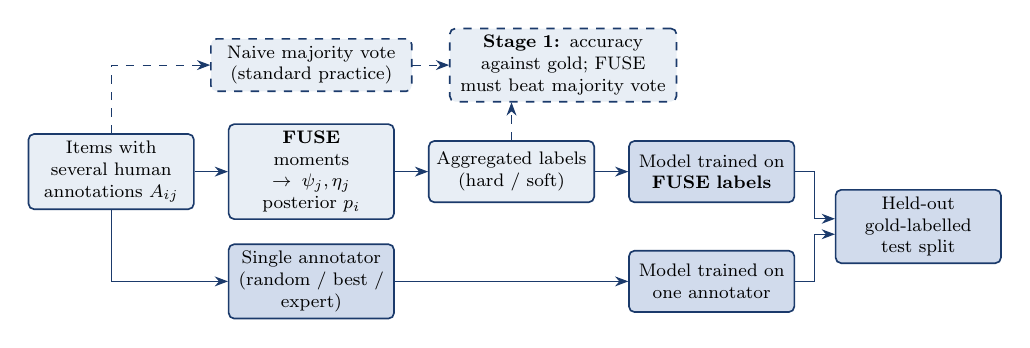
\begin{tikzpicture}[scale=0.82,transform shape,font=\fontsize{8}{9.6}\selectfont,>=Stealth,
 box/.style={draw=navy,rounded corners=2pt,align=center,text width=2.35cm,minimum height=0.95cm,inner sep=3pt,line width=0.6pt},
 st1/.style={box,fill=tblfill},st2/.style={box,fill=accent!22}]
\node[st1] (A) at (0,0) {Items with several human annotations $A_{ij}$};
\node[st1] (F) at (3.1,0) {\textbf{FUSE}\\moments $\to\psi_j,\eta_j$\\posterior $p_i$};
\node[st1] (L) at (6.2,0) {Aggregated labels\\(hard / soft)};
\node[st2] (M1) at (9.3,0) {Model trained on\\\textbf{FUSE labels}};
\node[st2] (S) at (3.1,-1.7) {Single annotator\\(random / best /\\expert)};
\node[st2] (M2) at (9.3,-1.7) {Model trained on\\one annotator};
\node[st2] (T) at (12.5,-0.85) {Held-out\\gold-labelled\\test split};
\node[st1,dashed,text width=2.9cm,minimum height=0.8cm] (MV) at (3.1,1.65) {Naive majority vote\\(standard practice)};
\node[st1,dashed,text width=3.3cm] (G) at (7.0,1.65) {\textbf{Stage 1:} accuracy against gold; FUSE must beat majority vote};
\draw[->,navy] (A)--(F); \draw[->,navy] (F)--(L); \draw[->,navy] (L)--(M1);
\draw[->,navy] (A.south) |- (S.west);
\draw[->,navy] (S)--(M2);
\draw[->,navy] (M1.east)--++(0.3,0) |- ([yshift=0.12cm]T.west);
\draw[->,navy] (M2.east)--++(0.3,0) |- ([yshift=-0.12cm]T.west);
\draw[->,navy,dashed] (A.north) |- (MV.west);
\draw[->,navy,dashed] (MV.east)--(G.west);
\draw[->,navy,dashed] (L.north)--(L.north |- G.south);
\end{tikzpicture}

\vspace{2pt}
{\itshape\fontsize{9}{11}\selectfont\textbf{Figure 1.} Study design. Light boxes: Stage 1; darker boxes: Stage 2. Stage 1 asks whether FUSE's labels are closer to gold than naive majority vote; Stage 2 compares a model trained on them with one trained on a single annotator's labels.\par}
\end{figure}

\textbf{Preliminaries.} Item $i$ has an unobserved label $y_i\in\{1,\dots,K\}$; annotator $j$ labels a subset of items, giving $A_{ij}$ or a missing entry. In the binary case, annotator $j$ has sensitivity $\psi_j$ and specificity $\eta_j$; under conditional independence given $y$ the off-diagonal covariance of $A$ is rank one with entries $\lambda_j\lambda_k$, where $\lambda_j\propto\psi_j+\eta_j-1$, so each $\lambda_j$ is identifiable from any three annotators. Multi-class tasks are handled one-vs-rest. FUSE's posterior $p_i$ is used as a hard label ($\arg\max$) or as a soft training target. A ``single expert'' means one annotator's label on every training item. Human annotators may violate conditional independence, since they share guidelines, biases and class priors, so independence is a risk to be measured, not assumed.

\subsection*{Stage 1 (until the midterm): does FUSE improve the aggregation decision?}

\begin{enumerate}[label=\alph*),leftmargin=18pt]
\item \lead{Data.} Two to three public datasets with several human annotations per item and a curated gold label, chosen from binary (textual entailment, Snow et al.\ [4]; relevance and sentiment sets from the Zheng et al.\ benchmark [5]) and multi-class (CIFAR-10H [6]; LabelMe [7]). Gold labels are hidden from every method and used only for scoring.
\item \lead{Implementation.} Implement FUSE from the paper and extend it to what human data needs: missing entries (the paper imputes missing scores as zero; we use pairwise-complete moments with a minimum-overlap rule), multi-class (the paper is binary only), and calibrated posteriors. Unit-test on simulated annotators with known $\psi_j,\eta_j$.
\item \lead{Aggregation benchmark (mandatory).} FUSE against naive majority vote (the standard practice and the main baseline to beat), Dawid--Skene and Jaffe et al.\ [2, 8] (baselines in the FUSE paper), on accuracy and log loss against gold. Annotations per item $k$ are subsampled to trace accuracy as a function of annotation budget.
\end{enumerate}

\textbf{Midterm criterion, fixed in advance.} On a dataset, Stage 1 succeeds if FUSE's accuracy gain over majority vote has a paired-bootstrap 95\% interval above zero at a stated $k$; on the study, if this holds on most datasets. ``FUSE beats majority vote only in regime X'' is a valid outcome, and Stage 2 then uses the best aggregator found.

\subsection*{Stage 2: does a model trained on FUSE labels beat a single expert's?}

A classifier (small CNN on image sets; pretrained encoder on a text set) is trained with identical architecture, optimiser and budget on labels from six arms:
\begin{itemize}
\item a single annotator, in three versions: a random annotator; the best annotator chosen by gold agreement (an optimistic bound for ``one expert''); the dataset's own expert where one exists;
\item naive majority vote (the standard practice);
\item Dawid--Skene;
\item FUSE hard labels and FUSE soft labels;
\item gold labels, as the ceiling.
\end{itemize}
Each arm is scored on a held-out gold-labelled test split no aggregator touched, by accuracy, log loss and calibration error over at least five seeds. Because several crowd labels cost more than one, the comparison is also made at equal annotation cost over a range of assumed expert-to-crowd price ratios, and the ratio where the advantage disappears is reported. \emph{Extension (gated on a Stage 2 gain):} feed the trained model back into FUSE as one more annotator.

\textbf{Evaluation discipline.} \emph{Leakage:} gold enters only in scoring, and hyperparameters are tuned on the single-annotator arm so FUSE is never the favoured arm. \emph{Circularity:} aggregated labels train on one item split and are tested on a disjoint one. \emph{Imperfect gold:} gold labels are noisy, so near-ceiling accuracy is not interpreted. \emph{Multiple comparisons:} results are paired bootstrap intervals over items, with every dataset, arm and $k$ reported, not the best cell. \emph{Observational limits:} datasets differ in annotator recruitment, so differences are described, not causally attributed.

\secrule{Objectives \& Deliverables}

\subsection*{Objectives}
\begin{itemize}
\item Adapt FUSE to human annotators: missing entries, multiple classes, calibrated posteriors.
\item Show, against gold and under the midterm criterion, whether FUSE improves label aggregation over standard methods and at which annotation budgets. This closes Stage 1.
\item Train models on FUSE labels and compare them with models trained on one expert, at equal items and at equal cost. This is the central contribution.
\end{itemize}

\subsection*{Deliverables}
\begin{itemize}
\item An open-source FUSE library with tests for missing data and multi-class tasks.
\item A reproducible benchmark: aggregation accuracy by $k$; Stage 2 metrics by arm with intervals.
\item A midterm presentation evaluating the Stage 1 criterion.
\item A final report stating, falsifiably, when FUSE labels beat a single expert's, when they do not, and the cost ratio at which the answer flips.
\end{itemize}

\secrule{Resources}

Public datasets only; Stage 1 runs on a laptop, Stage 2 on a single GPU. Advanced statistics, Python and a deep-learning framework are required; about half a day a week for an academic year. Academic project; any IP will be addressed when such occurs.

\secrule{Reference materials}

{\fontsize{8}{9.6}\selectfont
\setlength{\parskip}{1.5pt}\setlength{\parindent}{-12pt}\leftskip=12pt
[1] Lee, J., Ma, V., Zhao, S., Nair, Y., Spector, A., Cohen, R., Cand\`es, E. J. (2026). FUSE: Ensembling Verifiers with Zero Labeled Data. arXiv:2604.18547.\par
[2] Jaffe, A., Nadler, B., Kluger, Y. (2015). Estimating the accuracies of multiple classifiers without labeled data. AISTATS.\par
[3] Dawid, A. P., Skene, A. M. (1979). Maximum likelihood estimation of observer error-rates using the EM algorithm. J. Roy. Stat. Soc. C 28(1), 20--28.\par
[4] Snow, R., O'Connor, B., Jurafsky, D., Ng, A. Y. (2008). Cheap and fast---but is it good? Evaluating non-expert annotations for natural language tasks. EMNLP.\par
[5] Zheng, Y., Li, G., Li, Y., Shan, C., Cheng, R. (2017). Truth inference in crowdsourcing: Is the problem solved? PVLDB 10(5).\par
[6] Peterson, J. C., Battleday, R. M., Griffiths, T. L., Russakovsky, O. (2019). Human uncertainty makes classification more robust. ICCV.\par
[7] Rodrigues, F., Pereira, F. C. (2018). Deep learning from crowds. AAAI.\par
[8] Jaffe, A., Fetaya, E., Nadler, B., Jiang, T., Kluger, Y. (2016). Unsupervised ensemble learning with dependent classifiers. AISTATS.\par
}

\end{document}
